\section{Background}
\label{sec:background}

\subsection{Haskell}
\label{sec:haskell}

\begin{figure}
  \begin{equation*}
    \begin{split}
      expr\    \rightarrow\ & \texttt{Var}\ id                                       \\
                         |\ & \texttt{Lit}\ literal                                  \\
                         |\ & \texttt{App}\ expr\ expr                               \\
                         |\ & \texttt{Lam}\ \mathcal{L}\ expr                        \\
                         |\ & \texttt{Let}\ bind\ expr                               \\
                         |\ & \texttt{Case}\ expr\ \mathcal{L}\ \left[ alt \right]   \\
      id\      \rightarrow\ & \texttt{Local}\ \mathcal{L}                            \\
                         |\ & \texttt{Global}\ \mathcal{G}                           \\
      literal\ \rightarrow\ & \texttt{LitNum}\ \mathcal{N}                           \\
                         |\ & \texttt{LitStr}\ \mathcal{S}                           \\
      alt\     \rightarrow\ & ( altcon,\ [\mathcal{L}],\ expr )                      \\
      altcon\  \rightarrow\ & \texttt{DataAlt}\ \mathcal{G}                          \\
                         |\ & \texttt{LitAlt}\ literal                               \\
                         |\ & \texttt{Default}                                       \\
      bind\    \rightarrow\ & \texttt{NonRec}\ \mathcal{L}\ expr                     \\
                         |\ & \texttt{Rec}\ [ ( \mathcal{L},\ expr ) ]
    \end{split}
  \end{equation*}
  Where:
  \begin{tabular}[t]{l @{ $=$ } l}
    $\mathcal{S}$ & string literals    \\
    $\mathcal{N}$ & numeric literals   \\
    $\mathcal{L}$ & local identifiers  \\
    $\mathcal{G}$ & global identifiers
  \end{tabular}

  \caption{Simplified syntax of GHC Core in BNF style. $[]$ and $(,)$ denote repetition and grouping, respectively.}
  \label{fig:coresyntax}
\end{figure}

We decided to focus our theory exploration research on Haskell as it has mature, state-of-the-art implementations (\qspec{} \citep{QuickSpec} and \hspec{} \citep{claessen2013automating}). This is evident from the fact that the state-of-the-art equivalent for Isabelle/HOL, the \textsc{Hipster} \citep{Hipster} system, is actually implemented by translating to Haskell and invoking \hspec{}.

Haskell is a programming language which is well-suited to research; indeed, this was a goal of the language's creators \citep{marlow2010haskell}. Like most members of the \emph{functional programming} paradigm, Haskell is essentially a variant of $\lambda$-calculus; in fact an intermediate representation of the \textsc{GHC} compiler, known as \emph{GHC Core}, is based on a variant of the polymorphic $\lambda$-calculus known as \fc{}. For simplicity, we will focus on this Core language rather than the relatively large and complex syntax of Haskell proper. For a full treatment of \fc{} and its use in GHC, see \citep[Appendix C]{sulzmann2007system}.

The sub-set of Core we consider is shown in figure \ref{fig:coresyntax}; compared to the full language \footnote{As of GHC version 7.10.2, the latest at the time of writing.} our major changes are to erase types and use a custom representation of names. There are also several other forms of literal (machine words of various sizes, individual characters, etc.) which we omit for brevity, as their treatment is similar to those of strings and numerals.

\subsection{QuickCheck}
\label{sec:quickcheck}

Although unit testing is the de facto industry standard for quality assurance in non-critical systems, the level of confidence it provides is rather low, and totally inadequate for many (e.g. life-) critical systems. To see why, consider the following Haskell function, along with some unit tests (see \ref{sec:haskell} for more details on Haskell):

\begin{lstlisting}[language=Haskell, xleftmargin=.2\textwidth, xrightmargin=.2\textwidth]
factorial 0 = 1
factorial n = n * factorial (n-1)

fact_base      = factorial 0 == factorial 1
fact_increases = factorial 3 <= factorial 4
fact_div       = factorial 4 == factorial 5 `div` 5
\end{lstlisting}

The intent of the function is to map an input $n$ to an output $n!$. The tests check a few properties of the implementation, including the base case, that the function is monotonically increasing, and a relationship between adjacent outputs. However, these tests will \emph{not} expose a serious problem with the implementation: it diverges on half of its possible inputs!

All of Haskell's built-in numeric types allow negative numbers, which this implementation doesn't take into account. Whilst this is a rather trivial example, it highlights a common problem: unit tests are insufficient to expose incorrect assumptions. In this case, our assumption that numbers are positive has caused a bug in the implementation \emph{and} limited the tests we've written.

If we do manage to spot this error, we might capture it in a \emph{regression test} and update the definition of \hs{factorial} to handle negative numbers, e.g. by taking their absolute value:

\begin{lstlisting}[language=Haskell, xleftmargin=.2\textwidth, xrightmargin=.2\textwidth]
factorial 0 = 1
factorial n = let nPos = abs n
               in nPos * factorial (nPos - 1)

fact_neg = factorial 1 == factorial (-1)
\end{lstlisting}

However, this is \emph{still} not enough, since this function will also accept fractional values\footnote{Since we only use generic numeric operations, the function will be polymorphic with a type of the form \hs{forall t. Num t => t -> t}, where \hs{Num t} constrains the type variable \hs{t} to be numeric. In fact, Haskell will infer extra constraints such as \hs{Eq t} since we have used \hs{==} in the unit tests.}, which will also cause it to diverge. Clearly, by choosing what to test we are biasing the test suite towards those cases we've already taken into account, whilst neglecting the problems we did not expect.

Haskell offers a partial solution to this problem in the form of \emph{property checking}. Tools such as \qcheck{} separate tests into three components: a \emph{property} to check, which unlike a unit test may contain \emph{free variables}; a source of values to instantiate these free variables; and a stopping criterion. Here is how we might restate our unit tests as properties:

\begin{lstlisting}[language=Haskell, xleftmargin=.2\textwidth, xrightmargin=.2\textwidth]
fact_base        = factorial 0 == factorial 1
fact_increases n = factorial n <= factorial (n+1)
fact_div       n = factorial n == factorial (n+1) `div` (n+1)
fact_neg       n = factorial n == factorial (-n)
\end{lstlisting}

The free variables (all called \hs{n} in this case) are abstracted as function parameters; these parameters are implicitly \emph{universally quantified}, i.e. we've gone from a unit test asserting $factorial(3) \leq factorial(4)$ to a property asserting $\forall n, factorial(n) \leq factorial(n+1)$. Notice that unit tests like \hs{fact_base} are valid properties; they just assert rather weak statements.

To check these properties, \qcheck{} treats closed terms (like \hs{fact_base}) just like unit tests: pass if they evaluate to \hs{True}, fail otherwise. For open terms, a random selection of values are generated and passed in via the function parameter; the results are then treated in the same way as closed terms. The default stopping criterion for \qcheck{} (for each test) is when a single generated test fails, or when 100 generated tests pass.

The ability to state \emph{universal} properties in this way avoids some of the bias we encountered with unit tests. In the \hs{factorial} example, this manifests in two ways:

\begin{itemize}
  \item \qcheck{} cannot test polymorphic functions; they must be \emph{monomorphised} first (instantiated to a particular concrete type). This is a technical limitation, since \qcheck{} must know which type of values to generate, but in our example it would bring the issue with fractional values to our attention.

  \item The generators used by \qcheck{} depend only on the \emph{type} of value they are generating: since \hs{Int} includes positive and negative values, the \hs{Int} generator will output both. This will expose the problem with negative numbers, which we weren't expecting.
\end{itemize}

Property checking is certainly an improvement over unit testing, but the problem of tests being biased towards expected cases remains, since we are manually specifying the properties to be checked.

We can reduce this bias further through the use of \emph{theory exploration} tools, such as \qspec{} and \hspec{}. These programs \emph{discover} properties of a ``theory'' (e.g. a library), through a combination of brute-force enumeration, random testing and (in the case of \hspec{}) automated theorem proving.\footnote{See section \ref{sec:atp} for more information on automated theorem proving.}

\subsection{Theory Exploration}
\label{sec:theoryexploration}

\newcommand{\blank}{\cdot}

In this work we focus on the problem of \emph{(automated) theory exploration}, which includes the ability to \emph{generate} conjectures about code, to \emph{prove} those conjectures, and hence output \emph{novel} theorems without guidance from the user. The method of conjecture generation is a key characteristic of any theory exploration system, although all existing implementations rely on brute force enumeration to some degree.

We focus on \qspec{} \citep{QuickSpec}, which conjectures equations about Haskell code (these may be fed into another tool, such as \hspec{}, for proving). These conjectures are arrived at through the following stages:

\begin{enumerate}
  \item Given a typed signature $\Sigma$ and set of variables $V$, \qspec{} generates a list $terms$ containing the functions and constants from $\Sigma$, the variables from $V$ and type-correct function applications $f(x)$, where $f$ and $x$ are elements of $terms$. To ensure the list is finite, function applications are only nested up to a specified depth (e.g. 3).
  \item The elements of $terms$ are grouped into equivalence classes, based on their type.
  \item Each variable is instantiated to particular value, generated randomly by \qcheck{}.
  \item For each class, the members are compared (using a pre-specified function, such as equality \hs{==}) to see if these instantiations have caused an observable difference between members. If so, the class is split up to separate such members.
  \item The previous steps of variable instantiation and comparison are repeated until the classes stabilise (i.e. no differences have been observed for some specified number of repetitions).
  \item A set of equations are then conjectured, relating each class's members.
\end{enumerate}

Such $conjectures$ can be used in several ways: they can be simplified for direct presentation to the user (by removing any equation which is a can be derived from the others by rewriting), sent to a more rigorous system like \hspec{} or \textsc{Hipster} for proving, or even serve as a background theory for an automated theorem prover \citep{claessen2013automating}.

As an example, we can consider a simple signature for Peano numerals, addition and multiplication:

\begin{align*}
  \Sigma_{\mathbb{N}} = \{ & 0     && : \mathbb{N}, \\
                        & succ  && : \mathbb{N} \rightarrow \mathbb{N}, \\
                        & plus  && : \mathbb{N} \rightarrow \mathbb{N} \rightarrow \mathbb{N}, \\
                        & times && : \mathbb{N} \rightarrow \mathbb{N} \rightarrow \mathbb{N}\}
\end{align*}

Together with a set of variables, say $V_{\mathbb{N}} = \{x, y, z\}$, \qspec{}'s enumeration will resemble the following:

\begin{multline}
  terms_{\mathbb{N}} = \{0,\ succ,\ plus,\ times,\ x,\ y,\ succ(0),\ succ(x),\ succ(y),\ succ(z), \\
                    plus(0,\blank),\ plus(x, \blank),\ \dots \}
\end{multline}

Notice that our functions are curried, where $f(x,\blank)$ indicates \emph{partial application} of $f$ to $x$. This is required as the construction of $terms$ applies functions to one argument at a time.

These terms will be grouped into three classes, for $\mathbb{N}$, $\mathbb{N} \rightarrow \mathbb{N}$ and $\mathbb{N} \rightarrow \mathbb{N} \rightarrow \mathbb{N}$. As the variables $x$, $y$ and $z$ are instantiated to various randomly-generated numbers, these equivalence classes will be divided, until equations such as the following are conjectured (after simplification):

% To reproduce, run 'quickSpec nat' in haskell_example/src/QuickSpecExample.hs
\begin{align*}
                      plus(x, y) &= plus(y, x)
                      plus(x, 0) &= x
             plus(x, plus(y, z)) &= plus(y, plus(x, z))
                     times(x, y) &= times(y, x)
                     times(x, 0) &= 0
           times(x, times(y, z)) &= times(y, times(x, z))
                plus(x, succ(y)) &= succ(plus(x, y))
               times(x, succ(y)) &= plus(x, times(x, y))
            times(x, plus(y, y)) &= times(y, plus(x, x))
  plus(times(x, y), times(x, z)) &= times(x, plus(y, z))
\end{align*}

\qspec{} (and \hspec{}) is also compatible with Haskell's existing testing infrastructure, such that an invocation of \texttt{cabal test} can run these tools alongside more traditional QA tools like \qcheck{}, \textsc{HUnit} and \textsc{Criterion}.

In fact, there are similarities between the way a TE system like \qspec{} can generalise from checking \emph{particular} properties to \emph{inventing} new ones, and the way counterexample finders like \qcheck{} can generalise from testing \emph{particular} expressions to \emph{inventing} expressions to test. One of our aims is to understand the implications of this generalisation, the lessons that each can learn from the other's approach to term generation, and the consequences for testing and QA in general.

We attempt to mitigate the cost of running \qspec{}, by providing a machine learning layer analogous to that of premise selection in theorem proving. Of particular concern is the set of expressions $exprs$, which grows exponentially as the size of the expressions increases, and hence slows down the rest of the algorithm. Although complete, the current enumeration approach is wasteful: many combinations are unlikely to appear in theorems, which requires careful choice by the user of what to include in the signature. The key idea of premise selection is to make such choices automatically, by only including those expressions which are considered \emph{relevant} to the problem.

\iffalse TODO: Not immediately clear how the problem of reducing the set of expressions relates to premise selection \fi
\iffalse TODO: This detailed comparison with premise selection is opaque without defining/explaining what premise selection is \fi

\subsection{Clustering and Feature Extraction}
\label{sec:featureextraction}

Our approach to scaling up these Haskell theory exploration tools takes inspiration from two sources. The first is premise selection, which makes expensive algorithms used in theorem proving more practical by limiting the size of their inputs. We describe this approach in more details in \S \ref{sec:relevance}. Premise selection is a practical tool, used in production systems like the \emph{Sledgehammer} component of the Isabelle/HOL theorem prover.

Despite the idea's promise, we cannot simply invoke existing premise selection algorithms in our theory exploration setting. The reason is that theory exploration has no distinct \emph{goal} to compare expressions against. Instead, we are interested in relationships between \emph{any} terms generated from a signature, and hence we must consider the relevance of \emph{all terms} to \emph{all other terms}. A natural fit for such problems is \emph{clustering}, which attempts to group similar inputs together in an unsupervised way. See \S \ref{sec:clustering} for more information.

Our hypothesis is that clustering methods, as found in systems like ML4PG and ACL2(ml), can be used as relevance filters to break up large signatures into smaller ones more amenable to brute force enumeration.

\iffalse TODO: I would play up the clustering intelligence. Clustering is not just about breaking up, it is about discovering significant patterns in data. By forgetting this, you make motivation for your work sound too ``small'' \fi

Both of these approaches, premise selection and clustering, use \emph{machine learning} (ML) algorithms to analyse expressions, and hence rely on \emph{feature extraction} to transform the data into a suitable representation and remove irrelevant details. This has two benefits:

\begin{itemize}
  \item \emph{Feature vectors} (ordered lists of features) are chosen to represent the relevant information in a more compressed form than the raw data (for example, replacing descriptive identifier names with sequential numbers). This reduces the input size of the machine learning problem, improving efficiency (e.g. running time).
  \item We avoid learning irrelevant details, such as the text encoding system used, improving \emph{data} efficiency (the number of samples required to spot a pattern).
\end{itemize}

Another benefit of feature extraction is to \emph{normalise} the input data to a fixed-size representation. Many ML algorithms only work with inputs of a uniform size; feature extraction allows us to use these algorithms in domains where the size of each input is not known, may vary or may even be unbounded.

In our case, we will use a novel feature extraction algorithm, described in \S \ref{sec:recurrentclustering}, to transform expressions in Haskell Core into a fixed size representation, suitable for clustering via the standard \emph{k-means} algorithm.

\iffalse TODO: I have had a look now at section 5. I do not think feature extraction and clustering is explained/defined there, either. Seeing your contribution is feature extraction algorithms, you need to define feature vectors and clusters *here* \fi

\begin{figure}
  \centering
  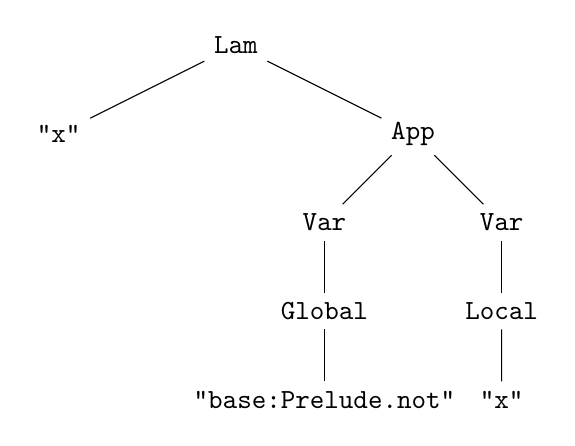
\begin{tikzpicture}[scale=0.75, level/.style={sibling distance=60mm/#1}]
      % Tree
      \node {\texttt{Lam}}
        child {node {\texttt{"x"}}}
        child {node {\texttt{App}}
          child {node {\texttt{Var}}
            child {node {\texttt{Global}}
              child {node {\texttt{"base:Prelude.not"}}}}}
          child {node {\texttt{Var}}
            child {node {\texttt{Local}}
              child {node {\texttt{"x"}}}}}};

      % Arrow
      %\node[single arrow,
      %      draw=black,
      %      fill=black!10,
      %      minimum height=2cm,
      %      shape border rotate=0] at (0,-1) {};
      %\draw[-latex] (A.east) -- (B.west);

      % Feature vector

  \end{tikzpicture}

  \caption{}

  \label{fig:featureextractionpic}
\end{figure}

\subsection{Clustering}
\label{sec:clustering}
% TODO
